\documentclass[12pt, letter]{article}

\usepackage[margin=0.8in]{geometry}
\usepackage{amsmath}
\usepackage{tikz}

\title{CS 381 - A3}
\author{Martin Mueller}
\date{Due: Friday, February $28^{th}$, 2020}

\begin{document}
	\maketitle
	\begin{enumerate}
		\item (10 points) Prove that there is a language $A \subseteq \{0,1\}^*$, with both of the following properties:
		\begin{enumerate}
			\item For all $x \in A$, $|x| \leq 5$.
			\item Every NFA that recognizes $A$ has more than $5$ states. Assume all NFAs here do not have $\lambda$-transitions.
		\end{enumerate}
		Hint: Do not explicitly define an example language. Count the number of NFAs that have a certain number of states and then count the number of languages that are comprised of binary strings of certain lengths and see what happens. Your proof will be "non-constructive".
		\begin{center}
			We start by explicitly defining the language $A$. Property (a) states that all elements in $A$ must be 5 or fewer characters in length. Since $A$ is a subset or equal to $\{0,1\}^{*}$, we could classify $A$ as the language containing all binary strings of lengths 0 to 5 or $\{\lambda,0,1,00,01,...,11111\}$. In order to construct an NFA that recognizes this language, we would need to make it accept every binary string of lengths 0 to 5. This would require at least 6 accept states, one for each character of its input with transitions in one direction from itself to a state accepting more characters. The last accept state, accepting any binary string of length 5 would not have any transitions and therefore the NFA would not accept any string of a length greater than 5. An example NFA would be:
\begin{center}
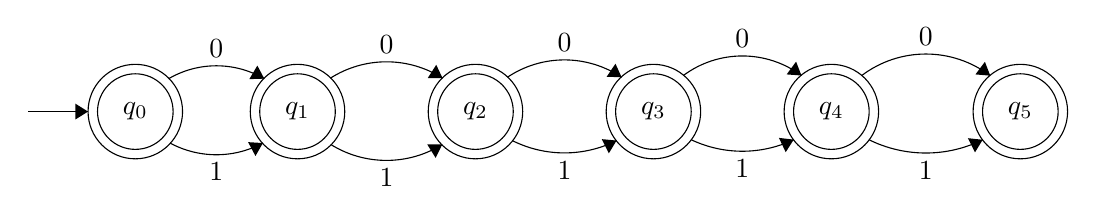
\begin{tikzpicture}[scale=0.2]
\tikzstyle{every node}+=[inner sep=0pt]
\draw [black] (11.3,-27) circle (3);
\draw (11.3,-27) node {$q_0$};
\draw [black] (11.3,-27) circle (2.4);
\draw [black] (21.6,-27) circle (3);
\draw (21.6,-27) node {$q_1$};
\draw [black] (21.6,-27) circle (2.4);
\draw [black] (32.9,-27) circle (3);
\draw (32.9,-27) node {$q_2$};
\draw [black] (32.9,-27) circle (2.4);
\draw [black] (44.2,-27) circle (3);
\draw (44.2,-27) node {$q_3$};
\draw [black] (44.2,-27) circle (2.4);
\draw [black] (55.5,-27) circle (3);
\draw (55.5,-27) node {$q_4$};
\draw [black] (55.5,-27) circle (2.4);
\draw [black] (67.5,-27) circle (3);
\draw (67.5,-27) node {$q_5$};
\draw [black] (67.5,-27) circle (2.4);
\draw [black] (4.5,-27) -- (8.3,-27);
\fill [black] (8.3,-27) -- (7.5,-26.5) -- (7.5,-27.5);
\draw [black] (19.399,-28.996) arc (-61.63756:-118.36244:6.208);
\fill [black] (19.4,-29) -- (18.46,-28.94) -- (18.93,-29.82);
\draw (16.45,-30.24) node [below] {$1$};
\draw [black] (30.785,-29.092) arc (-58.14121:-121.85879:6.697);
\fill [black] (30.79,-29.09) -- (29.84,-29.09) -- (30.37,-29.94);
\draw (27.25,-30.6) node [below] {$1$};
\draw [black] (13.413,-24.915) arc (120.32764:59.67236:6.014);
\fill [black] (19.49,-24.91) -- (19.05,-24.08) -- (18.54,-24.94);
\draw (16.45,-23.59) node [above] {$0$};
\draw [black] (23.686,-24.879) arc (122.5174:57.4826:6.631);
\fill [black] (30.81,-24.88) -- (30.41,-24.03) -- (29.87,-24.87);
\draw (27.25,-23.34) node [above] {$0$};
\draw [black] (34.925,-24.822) arc (123.87409:56.12591:6.504);
\fill [black] (42.18,-24.82) -- (41.79,-23.96) -- (41.23,-24.79);
\draw (38.55,-23.22) node [above] {$0$};
\draw [black] (46.096,-24.712) arc (126.67147:53.32853:6.285);
\fill [black] (53.6,-24.71) -- (53.26,-23.83) -- (52.66,-24.64);
\draw (49.85,-22.97) node [above] {$0$};
\draw [black] (57.414,-24.722) arc (127.24645:52.75355:6.752);
\fill [black] (65.59,-24.72) -- (65.25,-23.84) -- (64.65,-24.64);
\draw (61.5,-22.84) node [above] {$0$};
\draw [black] (41.859,-28.843) arc (-63.40771:-116.59229:7.392);
\fill [black] (41.86,-28.84) -- (40.92,-28.75) -- (41.37,-29.65);
\draw (38.55,-30.13) node [below] {$1$};
\draw [black] (53.111,-28.783) arc (-64.578:-115.422:7.597);
\fill [black] (53.11,-28.78) -- (52.17,-28.67) -- (52.6,-29.58);
\draw (49.85,-30.02) node [below] {$1$};
\draw [black] (65.112,-28.788) arc (-63.7085:-116.2915:8.155);
\fill [black] (65.11,-28.79) -- (64.17,-28.69) -- (64.62,-29.59);
\draw (61.5,-30.13) node [below] {$1$};
\end{tikzpicture}
\end{center}
			Since this NFA recognizes the language $A$, $A$ is also regular.
		\end{center}
		\item (10 points) For this problem, consider the language consisting of the set of all binary strings of the form $xbybz$, where $b \in \{0, 1\}$, $x,z \in \{0,1\}^{10}$ and $y \in \{0,1\}^*$. Show that this language is regular by constructing the smallest machine that you can think of that recognizes it. For fun (and a challenge), think about how many states will be required by any DFA that recognizes this language. \\ \\
		Give a digitally-drawn state diagram that is well-organized and the states have intuitive yet concise labels. \\ \\
		Give a concise and precise English description of how your machine works. If your machine has more than $10$ states, then you should describe your reasoning that led you to construct your particular machine (I'm not saying you should try to construct a machine with $10$ states or less). \\ \\
		Finally, give a formal description of your machine, contained in the file A3-2.nfa, that runs in the Automata-Simulator.
\begin{center}
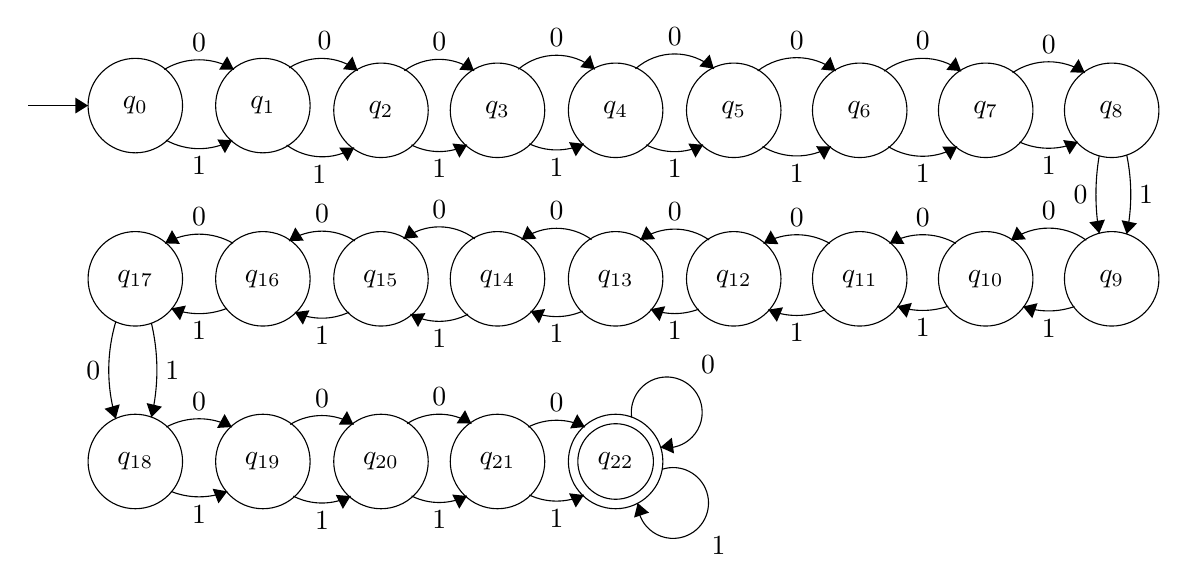
\begin{tikzpicture}[scale=0.2]
\tikzstyle{every node}+=[inner sep=0pt]
\draw [black] (8.7,-6.2) circle (3);
\draw (8.7,-6.2) node {$q_0$};
\draw [black] (16.8,-6.2) circle (3);
\draw (16.8,-6.2) node {$q_1$};
\draw [black] (24.3,-6.5) circle (3);
\draw (24.3,-6.5) node {$q_2$};
\draw [black] (31.7,-6.5) circle (3);
\draw (31.7,-6.5) node {$q_3$};
\draw [black] (39.2,-6.5) circle (3);
\draw (39.2,-6.5) node {$q_4$};
\draw [black] (46.7,-6.5) circle (3);
\draw (46.7,-6.5) node {$q_5$};
\draw [black] (54.7,-6.5) circle (3);
\draw (54.7,-6.5) node {$q_6$};
\draw [black] (62.7,-6.5) circle (3);
\draw (62.7,-6.5) node {$q_7$};
\draw [black] (70.7,-6.5) circle (3);
\draw (70.7,-6.5) node {$q_8$};
\draw [black] (70.7,-17.2) circle (3);
\draw (70.7,-17.2) node {$q_9$};
\draw [black] (62.7,-17.2) circle (3);
\draw (62.7,-17.2) node {$q_{10}$};
\draw [black] (54.7,-17.2) circle (3);
\draw (54.7,-17.2) node {$q_{11}$};
\draw [black] (46.7,-17.2) circle (3);
\draw (46.7,-17.2) node {$q_{12}$};
\draw [black] (31.7,-17.2) circle (3);
\draw (31.7,-17.2) node {$q_{14}$};
\draw [black] (39.2,-17.2) circle (3);
\draw (39.2,-17.2) node {$q_{13}$};
\draw [black] (24.3,-17.2) circle (3);
\draw (24.3,-17.2) node {$q_{15}$};
\draw [black] (16.8,-17.2) circle (3);
\draw (16.8,-17.2) node {$q_{16}$};
\draw [black] (8.7,-17.2) circle (3);
\draw (8.7,-17.2) node {$q_{17}$};
\draw [black] (8.7,-28.8) circle (3);
\draw (8.7,-28.8) node {$q_{18}$};
\draw [black] (16.8,-28.8) circle (3);
\draw (16.8,-28.8) node {$q_{19}$};
\draw [black] (24.3,-28.8) circle (3);
\draw (24.3,-28.8) node {$q_{20}$};
\draw [black] (31.7,-28.8) circle (3);
\draw (31.7,-28.8) node {$q_{21}$};
\draw [black] (39.2,-28.8) circle (3);
\draw (39.2,-28.8) node {$q_{22}$};
\draw [black] (39.2,-28.8) circle (2.4);
\draw [black] (1.9,-6.2) -- (5.7,-6.2);
\fill [black] (5.7,-6.2) -- (4.9,-5.7) -- (4.9,-6.7);
\draw [black] (14.847,-8.399) arc (-61.28896:-118.71104:4.365);
\fill [black] (14.85,-8.4) -- (13.91,-8.35) -- (14.39,-9.22);
\draw (12.75,-9.44) node [below] {$1$};
\draw [black] (22.596,-8.876) arc (-58.13813:-126.44309:3.822);
\fill [black] (22.6,-8.88) -- (21.65,-8.87) -- (22.18,-9.72);
\draw (20.39,-9.99) node [below] {$1$};
\draw [black] (10.54,-3.908) arc (121.13345:58.86655:4.275);
\fill [black] (14.96,-3.91) -- (14.53,-3.07) -- (14.02,-3.92);
\draw (12.75,-2.79) node [above] {$0$};
\draw [black] (18.472,-3.802) arc (122.56209:52.85669:3.811);
\fill [black] (22.82,-3.98) -- (22.49,-3.09) -- (21.89,-3.89);
\draw (20.71,-2.67) node [above] {$0$};
\draw [black] (25.789,-3.988) arc (126.31012:53.68988:3.733);
\fill [black] (30.21,-3.99) -- (29.86,-3.11) -- (29.27,-3.92);
\draw (28,-2.76) node [above] {$0$};
\draw [black] (33.02,-3.894) arc (130.28165:49.71835:3.759);
\fill [black] (37.88,-3.89) -- (37.59,-3) -- (36.95,-3.76);
\draw (35.45,-2.5) node [above] {$0$};
\draw [black] (40.459,-3.865) arc (131.56293:48.43707:3.754);
\fill [black] (45.44,-3.86) -- (45.17,-2.96) -- (44.51,-3.71);
\draw (42.95,-2.42) node [above] {$0$};
\draw [black] (48.225,-3.996) arc (127.50751:52.49249:4.064);
\fill [black] (53.17,-4) -- (52.84,-3.11) -- (52.24,-3.91);
\draw (50.7,-2.66) node [above] {$0$};
\draw [black] (56.256,-4.014) arc (126.85648:53.14352:4.074);
\fill [black] (61.14,-4.01) -- (60.8,-3.13) -- (60.2,-3.93);
\draw (58.7,-2.7) node [above] {$0$};
\draw [black] (64.406,-4.112) arc (123.66994:56.33006:4.137);
\fill [black] (68.99,-4.11) -- (68.6,-3.25) -- (68.05,-4.09);
\draw (66.7,-2.92) node [above] {$0$};
\draw [black] (69.906,-14.312) arc (-170.42971:-189.57029:14.81);
\fill [black] (69.91,-14.31) -- (70.27,-13.44) -- (69.28,-13.61);
\draw (69.2,-11.85) node [left] {$0$};
\draw [black] (64.312,-14.749) arc (125.68173:54.31827:4.095);
\fill [black] (64.31,-14.75) -- (65.25,-14.69) -- (64.67,-13.88);
\draw (66.7,-13.48) node [above] {$0$};
\draw [black] (56.596,-14.955) arc (119.62461:60.37539:4.257);
\fill [black] (56.6,-14.96) -- (57.54,-14.99) -- (57.04,-14.13);
\draw (58.7,-13.9) node [above] {$0$};
\draw [black] (48.597,-14.956) arc (119.60782:60.39218:4.257);
\fill [black] (48.6,-14.96) -- (49.54,-15) -- (49.05,-14.13);
\draw (50.7,-13.9) node [above] {$0$};
\draw [black] (40.767,-14.732) arc (125.00324:54.99676:3.806);
\fill [black] (40.77,-14.73) -- (41.71,-14.68) -- (41.14,-13.86);
\draw (42.95,-13.54) node [above] {$0$};
\draw [black] (33.229,-14.709) arc (125.81178:54.18822:3.796);
\fill [black] (33.23,-14.71) -- (34.17,-14.65) -- (33.59,-13.84);
\draw (35.45,-13.49) node [above] {$0$};
\draw [black] (25.743,-14.662) arc (127.30539:52.69461:3.724);
\fill [black] (25.74,-14.66) -- (26.68,-14.57) -- (26.08,-13.78);
\draw (28,-13.4) node [above] {$0$};
\draw [black] (18.46,-14.793) arc (123.008:56.992:3.836);
\fill [black] (18.46,-14.79) -- (19.4,-14.78) -- (18.86,-13.94);
\draw (20.55,-13.67) node [above] {$0$};
\draw [black] (10.588,-14.946) arc (120.10962:59.89038:4.31);
\fill [black] (10.59,-14.95) -- (11.53,-14.98) -- (11.03,-14.11);
\draw (12.75,-13.86) node [above] {$0$};
\draw [black] (7.461,-26.078) arc (-163.4647:-196.5353:10.817);
\fill [black] (7.46,-26.08) -- (7.71,-25.17) -- (6.75,-25.45);
\draw (6.51,-23) node [left] {$0$};
\draw [black] (10.668,-26.613) arc (118.38962:61.61038:4.379);
\fill [black] (14.83,-26.61) -- (14.37,-25.79) -- (13.89,-26.67);
\draw (12.75,-25.59) node [above] {$0$};
\draw [black] (18.537,-26.446) arc (121.35116:58.64884:3.868);
\fill [black] (22.56,-26.45) -- (22.14,-25.6) -- (21.62,-26.46);
\draw (20.55,-25.38) node [above] {$0$};
\draw [black] (25.959,-26.395) arc (122.67681:57.32319:3.781);
\fill [black] (30.04,-26.39) -- (29.64,-25.54) -- (29.1,-26.38);
\draw (28,-25.3) node [above] {$0$};
\draw [black] (29.768,-8.699) arc (-63.20779:-116.79221:3.922);
\fill [black] (29.77,-8.7) -- (28.83,-8.61) -- (29.28,-9.51);
\draw (28,-9.62) node [below] {$1$};
\draw [black] (37.182,-8.627) arc (-64.70861:-115.29139:4.053);
\fill [black] (37.18,-8.63) -- (36.24,-8.52) -- (36.67,-9.42);
\draw (35.45,-9.52) node [below] {$1$};
\draw [black] (44.757,-8.693) arc (-63.0772:-116.9228:3.991);
\fill [black] (44.76,-8.69) -- (43.82,-8.61) -- (44.27,-9.5);
\draw (42.95,-9.63) node [below] {$1$};
\draw [black] (52.868,-8.796) arc (-58.99597:-121.00403:4.21);
\fill [black] (52.87,-8.8) -- (51.93,-8.78) -- (52.44,-9.64);
\draw (50.7,-9.9) node [below] {$1$};
\draw [black] (60.883,-8.807) arc (-58.68245:-121.31755:4.2);
\fill [black] (60.88,-8.81) -- (59.94,-8.8) -- (60.46,-9.65);
\draw (58.7,-9.92) node [below] {$1$};
\draw [black] (68.551,-8.514) arc (-65.853:-114.147:4.525);
\fill [black] (68.55,-8.51) -- (67.62,-8.39) -- (68.03,-9.3);
\draw (66.7,-9.41) node [below] {$1$};
\draw [black] (71.655,-9.336) arc (11.68454:-11.68454:12.412);
\fill [black] (71.65,-14.36) -- (72.31,-13.68) -- (71.33,-13.48);
\draw (72.41,-11.85) node [right] {$1$};
\draw [black] (68.33,-18.963) arc (-70.74801:-109.25199:4.942);
\fill [black] (65.07,-18.96) -- (65.66,-19.7) -- (65.99,-18.75);
\draw (66.7,-19.74) node [below] {$1$};
\draw [black] (60.312,-18.941) arc (-71.13339:-108.86661:4.987);
\fill [black] (57.09,-18.94) -- (57.68,-19.67) -- (58.01,-18.73);
\draw (58.7,-19.71) node [below] {$1$};
\draw [black] (52.5,-19.161) arc (-66.97467:-113.02533:4.601);
\fill [black] (48.9,-19.16) -- (49.44,-19.93) -- (49.83,-19.01);
\draw (50.7,-20.03) node [below] {$1$};
\draw [black] (44.479,-19.125) arc (-69.1122:-110.8878:4.289);
\fill [black] (41.42,-19.13) -- (41.99,-19.88) -- (42.35,-18.94);
\draw (42.95,-19.91) node [below] {$1$};
\draw [black] (37.105,-19.254) arc (-66.37951:-113.62049:4.129);
\fill [black] (33.8,-19.25) -- (34.33,-20.03) -- (34.73,-19.12);
\draw (35.45,-20.1) node [below] {$1$};
\draw [black] (29.825,-19.446) arc (-61.98347:-118.01653:3.885);
\fill [black] (26.18,-19.45) -- (26.65,-20.26) -- (27.12,-19.38);
\draw (28,-20.4) node [below] {$1$};
\draw [black] (22.272,-19.317) arc (-64.92609:-115.07391:4.062);
\fill [black] (18.83,-19.32) -- (19.34,-20.11) -- (19.76,-19.2);
\draw (20.55,-20.2) node [below] {$1$};
\draw [black] (14.521,-19.075) arc (-68.4145:-111.5855:4.813);
\fill [black] (10.98,-19.08) -- (11.54,-19.83) -- (11.91,-18.9);
\draw (12.75,-19.91) node [below] {$1$};
\draw [black] (9.722,-20.013) arc (13.3337:-13.3337:12.951);
\fill [black] (9.72,-25.99) -- (10.39,-25.32) -- (9.42,-25.09);
\draw (10.57,-23) node [right] {$1$};
\draw [black] (14.539,-30.697) arc (-67.99906:-112.00094:4.776);
\fill [black] (14.54,-30.7) -- (13.61,-30.53) -- (13.98,-31.46);
\draw (12.75,-31.54) node [below] {$1$};
\draw [black] (22.366,-31) arc (-62.88802:-117.11198:3.984);
\fill [black] (22.37,-31) -- (21.43,-30.92) -- (21.88,-31.81);
\draw (20.55,-31.94) node [below] {$1$};
\draw [black] (29.757,-30.99) arc (-63.43907:-116.56093:3.93);
\fill [black] (29.76,-30.99) -- (28.82,-30.9) -- (29.27,-31.8);
\draw (28,-31.91) node [below] {$1$};
\draw [black] (33.647,-26.611) arc (116.82686:63.17314:3.994);
\fill [black] (37.25,-26.61) -- (36.76,-25.8) -- (36.31,-26.7);
\draw (35.45,-25.68) node [above] {$0$};
\draw [black] (37.182,-30.927) arc (-64.70861:-115.29139:4.053);
\fill [black] (37.18,-30.93) -- (36.24,-30.82) -- (36.67,-31.72);
\draw (35.45,-31.82) node [below] {$1$};
\draw [black] (40.218,-25.99) arc (187.82394:-100.17606:2.25);
\draw (44.6,-22.66) node [right] {$0$};
\fill [black] (42.05,-27.9) -- (42.91,-28.29) -- (42.77,-27.29);
\draw [black] (42.147,-29.297) arc (108.16235:-179.83765:2.25);
\draw (45.26,-34.13) node [right] {$1$};
\fill [black] (40.6,-31.44) -- (40.37,-32.36) -- (41.32,-32.05);
\end{tikzpicture}
\end{center}
		\begin{center}
			The machine starts at $q_{0}$. From there, it must be given a string in $\{0,1\}^{22}$ in order to reach the accept state. From there, any further input will just cause it to remain in the accept state. It's designed this way because $xbybz$ is effectively:
			\begin{align*}
				xbybz &= \{0,1\}^{10}\{0,1\}\{0,1\}^{*}\{0,1\}\{0,1\}^{10} \\
				&= \{0,1\}^{11}\{0,1\}^{*}\{0,1\}^{11}
			\end{align*}
			As far as this DFA goes, this means that it needs to accept somewhere between 22 and infinite zeros or ones. It's pretty repetitive, so it's easy to prove this is the case.
		\end{center}
	\end{enumerate}
\end{document}